\chapter{Introducción}
\label{chap:introduccion}

\lettrine{A}{partir} de la segunda década de los 2000, las redes sociales han experimentado
un crecimiento continuado de su uso, tanto en número de usuarios como en
cantidad de información generada. Como se muestra en el informe \textit{Digital 2023 Global Overview Report} (We Are Social et al., 2023)
\cite{wearesocial}, a principios del año 2013 existían alrededor de 1.700 millones de usuarios en las redes sociales,
mientras que a principios del año 2023, esta cifra aumentó hasta los 4.700 millones, con una variación anual media del 10,8\% (se puede ver
más información en la Figura \ref{fig:usuarios_redes_sociales}).
Así, plataformas como Facebook, Instagram, Twitter o YouTube, cuentan con millones de usuarios activos diariamente,
donde se comparte información o se crea contenido de entretenimiento. Además, las redes sociales se han convertido en
un lugar donde se debate sobre temas políticos, sociales o económicos, y donde se comparten diversas opiniones y noticias.
Este hecho se puede ver, de nuevo, en el informe mecionado anteriormente, donde se muestra que el 34,2\% de los usuarios
de redes sociales las utilizan para informarse sobre noticias, el 28,8\% para saber cuáles son los temas de actualidad
y el 23,4\% para compartir opiniones y debatir con otros usuarios.

\bigskip
\begin{figure}[H]
	\centering
	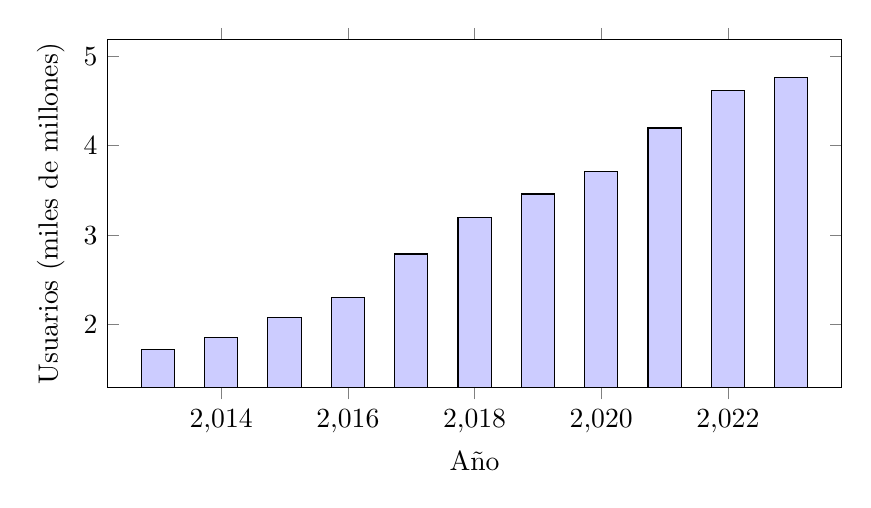
\begin{tikzpicture}
		\begin{axis}[
				width=0.9\textwidth,
				height=6cm,
				xmajorgrids=false,
				ylabel=Usuarios (miles de millones),
				xlabel=Año,
				ybar=6pt,
				bar width=12pt,
				enlarge x limits=0.08,
				enlarge y limits=0.14,
			]
			\addplot[fill=blue!20]
			coordinates {(2013,1.720) (2014,1.857) (2015,2.078)
					(2016,2.307) (2017,2.789) (2018,3.196) (2019,3.461)
					(2020,3.709) (2021,4.199) (2022,4.623) (2023,4.760)};
		\end{axis}
	\end{tikzpicture}
	\caption{Evolución del número de usuarios en redes sociales}
	\label{fig:usuarios_redes_sociales}
\end{figure}

\section{Importancia de las redes sociales}
\label{sec:intr_importancia}
Toda esta información generada tiene una gran relevancia a distintos niveles. En primer lugar, cabe destacar el impacto que
tienen las redes sociales a nivel político. Y es que en la actualidad, vivimos en una campaña permanente (Blumenthal, 1980)
\cite{sydney1980permanent},
donde el acceso a estas plataformas ofrece la posibilidad a los ciudadanos de estar informados sobre política, mientras que a las instituciones
de poder les permite conocer el estado de la opinión pública (Strömbäck, 2008)
\cite{stromback2008four}, pudiendo llegar a influenciar "mucho" o "bastante" la intención de voto (Gallardo-Paúls, 2016) \cite{gallardo2016pseudopolitica}.
En segundo lugar, el contenido que se genera en las redes sociales es de gran relevancia a nivel sociológico ya que sirve para analizar, entre muchas cosas,
la representación que tienen en ellas la sociedad o la forma en la que interactuamos (Mislove et al., 2011) \cite{mislove2011understanding}. Cabe resaltar también la influencia
que tienen las plataformas digitales a nivel económico, ya que se han convertido en un lugar donde las empresas
publicitan sus productos y servicios y a las que destinan gran parte de sus presupuestos en publicidad
(Saxena et al., 2013) \cite{saxena2013advertising}. Finalmente, destacar el rol fundamental que juega la seguridad en las redes sociales,
ya que se han convertido en lugares donde se comparte información personal, y donde se pueden cometer delitos como
el \textit{cyberbullying} o el \textit{grooming} (Machimbarrena et al., 2018) \cite{machimbarrena2018internet}.

\section{Perfilado de autor}
\label{sec:intro_perfilado}

El perfilado de autor, también conocido como perfilado de usuario o \textit{author profiling} en inglés, consiste en determinar, a partir de un texto,
las características de su autor, como su género, edad, rasgos personales, etc. Para ello se hace uso de diversas técnicas de aprendizaje automático
basadas en el procesado del lenguaje natural (\textit{Natural Language Processing} o NLP en inglés), que permiten extraer características lingüísticas del texto y utilizarlas para una
posterior clasificación.

\bigskip
De esta forma, el perfilado de autor en redes sociales se ha convertido en un área de investigación de gran interés
en los últimos años, posicionándose como una herramienta de creciente importancia en campos como la seguridad, el \textit{marketing}
o la investigación forense (Rangel et al., 2013) \cite{rangel2013overview}. Así, la evolución y el perfeccionamiento del perfilado de autor propiciaría la creación de
una herramienta de gran ayuda para los sociólogos a la hora de realizar análisis sobre temas que dispongan de información digital;
ofrecería a las empresas  una forma de conocer el perfil de los clientes que opinan de
forma positiva y negativa de sus productos; tendría un gran valor
para los partidos políticos, dado que podrían conocer cuál es el perfil de sus votantes; y respaldaría el trabajo de los cuerpos de seguridad
a la hora de la evaluación de sospechosos en base a su perfil lingüístico.

\section{Objetivos del trabajo}
\label{sec:intro_objetivos}

Tras la introducción al perfilado de autor y las motivaciones que existen para su estudio a nivel de las redes sociales,
se expondrán a continuación los objetivos principales de este trabajo.

\bigskip
El primero de ellos es la investigación del estado del arte del perfilado automático de autor, enmarcado en
el análisis de documentos digitales. Para acotar
el estudio, la investigación se centrará en el perfilado de autor en el ámbito de la lengua inglesa y se priorizarán
aquellos algoritmos que perfilen los rasgos generacionales del autor.
Asimismo, se profundizará en cuáles son las técnicas de aprendizaje automático más utilizadas en el campo,
cuáles son las características que se extraen comúnmente y cuáles son los algoritmos que mejores resultados obtienen.

\bigskip
Como segundo objetivo, una vez se hayan logrado ejecutar satisfactoriamente los algoritmos seleccionados tras el estudio,
se pretende desarrollar una aplicación que permita a los usuarios el perfilado automático de una serie de características
demográficas de una colección de textos, mostrando un tablero web visual de datos (\textit{dashboard} en inglés) accesible y usable con los resultados obtenidos.
Además, se liberará el código de la aplicación en un repositorio público de GitHub \cite{github}, para que pueda ser utilizado de forma
gratuita por cualquier persona y pueda crecer gracias a la colaboración de la comunidad.

\bigskip
Por último, empleando la aplicación previamente desarrollada, se utilizará como caso de uso la colección sobre el movimiento
\textit{Black Lives Matter} (\#BLM) proporcionada para este TFG. Se busca, por lo tanto, realizar un análisis con un componente sociológico
de los perfiles obtenidos,
con el objetivo de obtener conclusiones acerca del movimiento y de los usuarios que participaron debatiendo sobre el mismo en las redes sociales.

\bigskip
Se trata, en definitiva, de un trabajo que pretende profundizar en el perfilado de autor, tanto desde un punto de vista teórico como práctico,
haciendo accesible mediante la creación de una aplicación, una herramienta basada en técnicas de aprendizaje automático, y
demostrando su utilidad con el análisis de un fenómeno social de gran relevancia.

\section{Estructura de la memoria}
\label{sec:intro_estructura}

La memoria se estructura en diez capítulos, que se describen a continuación:

\begin{itemize}
	\item \textbf{Introducción}: Se trata del capítulo actual; en él se contextualiza el perfilado automático de autores junto a su utilidad
		para el análisis de la información generada en las redes sociales. Asimismo, se exponen los objetivos que tiene este trabajo y la estructura
		de esta memoria.
	
	\item \textbf{Estado del arte del perfilado de autor}: En este capítulo se realiza una revisión bibliográfica desde los inicios del perfilado de autor y se explican
		los conceptos básicos que se utilizan habitualmente en el campo. Posteriormente, se analizan las tareas sobre el perfilado de autor que se han llevado a cabo,
		seleccionando y evaluando diferentes algoritmos presentados en las mismas.

	\item \textbf{Herramientas, técnicas y lenguajes}: Tercer capítulo de la memoria, donde se exponen las herramientas utilizadas en todo el proceso de desarollo
		y se argumenta la elección de cada una de ellas.

	\item \textbf{Metodología}: En este capítulo se explica la metodología que se ha seguido para el desarrollo de la aplicación, así como
		los roles que desempeña cada uno de los miembros del equipo junto a las adaptaciones que se han realizado a la metodología propuesta.

	\item \textbf{Análisis}: A lo largo de este capítulo se detallan los requisitos funcionales y no funcionales identificados para la aplicación.
	
	\item \textbf{Diseño}: En este capítulo se muestran los diagramas de arquitectura y de clases diseñados, así como los prototipos de la interfaz web de usuario.

	\item \textbf{Implementación}: Séptimo capítulo de la memoria; en él se explica a bajo nivel las adaptaciones que fueron necesarias para integrar los algoritmos
		seleccionados en la aplicación. Además, se detalla la estructura de directorios del proyecto y se justifica la decisión de liberar el código fuente.

	\item \textbf{Caso de uso \#BLM}: En este capítulo se utiliza como ejemplo de caso de uso de la aplicación el análisis de la colección de referencia ofrecida para este TFG
		sobre el movimiento \textit{Black Lives Matter}.

	\item \textbf{Planificación y costes}: A lo largo de este capítulo se explican las tareas realizadas en cada \textit{sprint} y se desglosan los costes
		económicos del proyecto.

	\item \textbf{Conclusiones}: Capítulo final de la memoria, en el que se exponen las líneas de trabajo futuras y se realiza una valoración de los conocimientos
		adquiridos durante todo el proceso.

\end{itemize}

